\chapter{Background Theory} \label{chap:background-theory}
This chapter will focus on general level set methods: how to derive them and we will present some key features. In addition we include some theory on distance functions which is useful for level set methods in general, but will prove especially relevant for our application. Finally, we look at shape derivatives, or more specific, derivatives of domain integrals and how they can are utilized as a tool for modeling the level set formulation to a specific application.


\section{Level Set Methods}\label{sec:levelset-methods}
Before we begin, we must clarify that all derivations in this section will be performed for curves in $\realspacem^2$, but everything can be extended to surfaces in a multidimensional space $\realspacem^n$. This is simply a choice to be consistent with the modeling and implementation which is only applied to curves in this thesis.

A two-dimensional level set formulation is an implicit representation of a closed curve or curves. The curve is described by a higher dimensional function by being a level curve for some constant value. We explain this concept through a familiar example for most of us, namely level curves on a map. Provided a continuous function of the ground surface elevation on an area, the level contours or curves join points on the surface of equal elevation. All curves representing the same value, or elevation in the cartographic setting, are called \textit{iso-curves} or \textit{iso-contours}. On a map, there are numerous iso-curves of different values separated by a constant height. Such contours are thus effectively describing the steepness and height, and thus the shape of the ground in the area. In a level set context, we are not interested in the shape of the underlying higher dimensional function in the same way. We look at a single iso-value, which by standard practice is the zero iso-value, which yields a curve called the \textit{zero iso-contour}. The corresponding zero iso-contour(s) will split the domain into regions of two types: one where the underlying function is positive and one where it is negative. Level set methods track the shape of these curves and how they change over time. 


\subsection{Implicit Derivation}
Now that we have an intuition about iso-curves, we can discuss the principle of the level set method. The goal is to represent a closed curve or surface, \curve, that moves under the influence of a velocity field that can change over time, \velocityfield. We will from now on use bold face letters for vectors and $\vv{v}$ denotes a vector field $v$. The level set approach to this problem, as first presented in 1987 by S.Osher and J. Sethian \cite{Osher-Sethian}, is to define a continuous function \uxt\ defined on a domain $\domainm \in \realspacem^2$ containing the initial curve $\Gamma|_{t=0}$. The domain \domain\ is split into two parts by the curve \curve, the interior $\Omega$, and the exterior  $\domainm \setminus \Omega$. See \figref{fig:levelset-representation} as a reference.
\begin{figure}
    \centering
    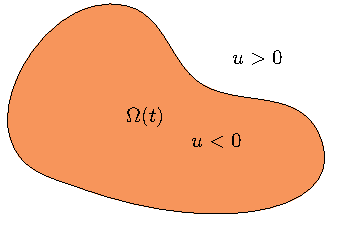
\includegraphics[width=.5\linewidth]{figures/tikz-figures/optimization-problem.tex}
    \caption[Level set function]{Level set representation of a curve \curve.}
    \label{fig:levelset-representation}
\end{figure}
The function \uxt\ must be constructed in a way that satisfies the following properties
\begin{align}
    u(\mathbf{x}, t) < 0 \qquad &\text{for } \mathbf{x} \in  \Omega(t) \label{eq:interior}\\
    u(\mathbf{x}, t) = 0 \qquad &\text{for } \mathbf{x} \in  \curvem \label{eq:zero-iso-curve}\\
    u(\mathbf{x}, t) > 0 \qquad &\text{for } \mathbf{x} \in  \mathcal{D} \setminus \Omega(t) \label{eq:exterior}.
\end{align}
Now, the curve \curve\ can be described in terms of \uxt\ by being its zero iso-contour. This means that if we can find the proper evolution of 
\uxt\ we can implicitly track the motion of the curve.
Now, what we need is to find a model for the change in \uxt\ in order
to simulate the level curve, \curve, as a curve flowing in the velocity field \velocityfield. Because the zero iso-curve of \uxt\ is the only region of interest, we differentiate \eqref{eq:zero-iso-curve} with respect to time and thus, assuming that $\uxtm$ is at least in $C^1(\curvem)$, the following must hold.
\begin{equation}
    \bigg(u(\mathbf{x}, t)_t + \nabla u(\mathbf{x}, t) \, \frac{\partial \mathbf{x}}{\partial t} \bigg)_{\mathbf{x}\in \curvem} = 0.
    \label{eq:general-u-flow}
\end{equation}
The term $\mathbf{x}_t=\frac{\partial \mathbf{x}}{\partial t}$ for $\mathbf{x} \in \curvem$ is the velocity of the curve. The curve only represents a shape or boundary of a domain and has thus no density. Hence, the only component of the velocity that has any influence on the movement is the normal component. We define positive direction of speed to be inwards and define the normal vector $\vv{n}_{\curvem}$ pointing out of $\Omega(t)$. Thus the velocity for the zero level curve $\mathbf{x}_t$ must be
\begin{equation}
    \mathbf{x}_t = (\velocityfieldm \cdot \vv{n}_{\curvem})\cdot \vv{n}_{\curvem}= -v_n \vv{n}_{\curvem}.
    \label{eq:velocity-levelcurve}
\end{equation}
We can also see from \eqref{eq:interior}-\eqref{eq:exterior} that the gradient of \uxt\ at the curve \curve\ is always pointing in the direction of the normal vector of \curve, $\vv{n}_{\curvem}$. Thus we can write the normal vector as
\begin{equation}
    \vv{n}_{\curvem} = \frac{\nabla u}{|\nabla u|}.
    \label{eq:normal-of-levelcurve}
\end{equation}

Inserting \eqref{eq:velocity-levelcurve} and \eqref{eq:normal-of-levelcurve} into \eqref{eq:general-u-flow}, we get the levelset evolution equation 

\begin{tcolorbox}[title=The level set evolution equation]
\begin{equation}
    u_t - v_n\, |\nabla u| = 0
    \label{eq:general-level-set}
\end{equation}
\end{tcolorbox}

We constructed this partial differential equation to let the curve, \curve, flow in 
our velocity field, \velocityfield, and have laid no restrictions on the rest of the higher dimensional curve
\uxt. However, we see that we could have done exactly the same for 
any other iso-value of \uxt\ by defining 
\begin{align*}
    u(\mathbf{x}, t) < k \qquad &\text{for } \mathbf{x} \in  \Omega_k(t) \\
    u(\mathbf{x}, t) = k \qquad &\text{for } \mathbf{x} \in  \Gamma_k(t) \\
    u(\mathbf{x}, t) > k \qquad &\text{for } \mathbf{x} \in  \mathcal{D} \setminus \Omega_k(t) .
\end{align*}
and differentiating the iso-curve with respect to time. Because the right hand 
side $k$ is only a constant, this would make no difference to the resulting PDE. Thus
it is not only the zero iso-contour, but the entire function \uxt\ that is transported 
in the velocity field \velocityfield.

We will now show that this implicit formulation will yield the same solution as explicitly tracking the curve moving with the given velocity provided by the velocity field. The strategy was proposed by Osher and Sethian in the paper from 1988, which introduced level set methods. Given a parametric curve with a given speed, we can track its position through the equations of motion and show through a reformulation that this yields the same general level set equation.

\subsection{Explicit Derivation} \todo{burde jeg endre alle x til x1 og y til x2? Jeg bruker jo vektor-x ellers?}
We begin with a closed initial curve $\Gamma_0$ that moves along in the normal direction with speed $v_n=v_n(\mathbf{x}, t)$ for $\mathbf{x}\in \Gamma$. Given a non-zero velocity, the curve moves over time and let then \curve\ be the set of curves for $t\in[0, \infty]$. In an explicit formulation, every curve $\Gamma(t)$ can be parameterized by a variable $s\in[0, S]$ and let the parameterized position vectors be denoted $\mathcal{C}(s, t) = (x(s, t), y(s, t))$ for every curve in \curve. For a fixed $s=s^*$ this can be viewed as a Lagrangian perspective, following a certain particle moving with speed $v_n$. Fixing the time $t=t^*$ yields the parameterized curve $\mathcal{C}(s, t^*) = \Gamma(t^*)$.

The tangent vector field with respect to the curve, $\vv{T}(\mathcal{C})$ comes easily from the parameterization by derivation with of $x$ and $y$ respect to $s$:
\begin{equation*}
    \vv{T}(\mathcal{C}) =  \begin{bmatrix}x_s \\ y_s \end{bmatrix}
\end{equation*}
Since the unit normal is orthogonal to the tangent, we write it as
\begin{equation}
    \vv{n}(\mathcal{C}) = \frac{1}{\sqrt{x_s^2+y_s^2}}\begin{bmatrix}y_s \\ -x_s \end{bmatrix}.
    \label{eq:parametric-normal}
\end{equation}
We now get the equations of motion for a curve moving with a known speed $v_n$ in the normal direction,

\begin{equation}
    \mathcal{C}(s, t)_t = \begin{bmatrix}x_t \\ y_t \end{bmatrix} = v_n \vv{n} = \frac{v_n}{\sqrt{x_s^2+y_s^2}}\begin{bmatrix}y_s \\ -x_s \end{bmatrix}.
    \label{eq:parametric-motion-equations}
\end{equation}

The function $\mathcal{C} : [0, S]\times [0, \infty) \to \realspace^2$ forms a continuous mapping from $(t, s) \to (x, y)$. The Jacobi matrix of this mapping is defined by the relations 
\begin{align*}
    dx &= x_s\, ds + x_t\,dt  \\ %\label{eq:parametric-jacobi-dx}
    dy &= y_s \, ds + y_t\, dt . %\label{eq:parametric-jacobi-dy}
\end{align*}
Which on matrix form is
\begin{equation}
    \begin{bmatrix} dx \\ dy \end{bmatrix} = J \cdot \begin{bmatrix} ds \\dt \end{bmatrix} = \begin{bmatrix}
    x_s & x_t \\ y_s & y_t
    \end{bmatrix} \cdot \begin{bmatrix} ds \\dt \end{bmatrix}.
    \label{eq:parametric-jacobi-relation}
\end{equation}

The determinant of the Jacobi matrix, called the Jacobian, is thus
\begin{equation}
    |J|= x_s y_t - x_t y_s = v_n \frac{-x_s^2 - y_s^2}{\sqrt{x_s^2+y_s^2}} = -v_n \sqrt{x_s^2+y_s^2}, 
    \label{eq:jacobi-velocity-relation}
\end{equation}
where we have used \eqref{eq:parametric-motion-equations} for the relations between $(x_t, y_t)\to (x_s, y_s)$. 

As long as the Jacobian is non-zero at a given point, the inverse mapping theorem claims that there exists an inverse mapping locally around the point. That is indeed the case here as long as the normal speed $v_n$ is non-zero and the parameterization is chosen so that we avoid $x_s=y_s=0$ at the same time.

\begin{figure}
    \centering
    \includegraphics{figures/tikz-figures/t-fxy.tex}
    \caption[Zero level curves over time]{A representation of the function $t=f(x, y)$ for some curves in the set of curves \curve.}
    \label{fig:t-functionxy}
\end{figure}

Hence, there will locally exist an inverse mapping $\mathcal{C}^{-1} : (x, y) \to (t, s)$ such that there exists a relation $t=f(x, y)$. An example of how this function can look is displayed in \figref{fig:t-functionxy}. Here we can see that this function is well defined if a curve does not cross the same spatial point more than once. This is fulfilled if the speed function is continuous and non-zero. The function $f(x, y)$ can thus be used to implicitly describe the set of curves \curve\ by its iso-contours. 

Using this, we can transform \eqref{eq:parametric-motion-equations} into a PDE governing the motion of the curve.
\begin{proposition}
    The inverse mapping $t=f(x, y)$ must satisfy 
    \begin{equation}
        v_n^2(f_x^2 + f_y^2) = 1,
        \label{eq:parametric-PDE}
    \end{equation}
    for a non-zero $v_n\in C^0$.
    \label{prop:parametric-PDE}
\end{proposition}
\begin{proof}
The total derivative of $t$, $dt$, can be written in two ways. 
\begin{align}
    dt &= t_x dx + t_y dy  \label{eq:dt-1}\\
    dt &= \frac{1}{|J|}(y_s dx - x_s dy) \label{eq:dt-2},
\end{align}
\eqref{eq:dt-1} is the total derivative, and \eqref{eq:dt-2} comes from \eqref{eq:parametric-jacobi-relation} solved for $dt$. By comparing \eqref{eq:dt-1} and \eqref{eq:dt-2} we get that the terms in front of $dx$ and $dy$ have to be equal. 
\begin{equation}
    t_x = \frac{y_s}{|J|}, \qquad t_y = -\frac{x_s}{|J|}
    \label{eq:t-jacobian}
\end{equation}

Using also the relation between the Jacobian and the normal velocity from \eqref{eq:jacobi-velocity-relation}, we get
\begin{equation*}
    f_x^2+f_y^2 = t_x^2+t_y^2 = \frac{y_s^2 + x_s^2}{|J|^2} = \frac{1}{v_n^2}.
\end{equation*}
\end{proof}

The partial differential equation \eqref{eq:parametric-PDE} can be solved for $(x, y, f)$ and is for all spacial points $(x, y)$ the time $t = f(x, y)$ at which the curve passed through the point. We can see from \eqref{eq:t-jacobian} that given the parameterization of the initial curve, all the information needed to solve \eqref{eq:parametric-PDE} is possible to obtain from the initial curve. The PDE in \eqref{eq:parametric-PDE} is then a well-defined boundary value problem. We can find the entire three dimensional surface described by $f(x, y)=t$ only from its boundary where $f(x, y)=0$.

We now prove that the solution of \eqref{eq:parametric-PDE} will yield the same solution as the level set evolution equation \eqref{eq:general-level-set}. 
\begin{comment}
Consider a small enough section of the curve, \curve, for a fixed $t=t^*$, such that the function is not multivalued with respect to $y$. This curve section can thus be denoted as $y=Y(x, t)$. Inserting this back into \eqref{eq:parametric-PDE}, we obtain \todo{igjen: hvordan?}
\begin{equation}
    Y_t - v_n(1+Y_x^2)^{1/2} = 0,
\end{equation}
which is a Hamilton-Jacobi equation. \todo{ref+er det restriksjoner på vn?} 
\end{comment}
The trick to reformulate this into an implicit formulation is, as we did for the implicit derivation, to define a higher dimensional function \uxt\ satisfying \eqref{eq:interior}-\eqref{eq:exterior}. The level curves of this function is defined by $\uxtm=\text{const}$ and we still have that $t=f(x, y)$. This means that in two dimensions, $u = u(x, y, f(x, y))$.

\begin{align*}
    0 &= \frac{\diff u}{\diff x} = u_x+u_t f_x \\
    0 &= \frac{\diff u}{\diff y} = u_y+u_t f_y
\end{align*}
 And we directly get the relations
\begin{equation}
    f_x = \frac{-u_x}{u_t}, \qquad f_y = \frac{-u_y}{u_t},
    \label{eq:f-u-relations}
\end{equation}
Inserting \eqref{eq:f-u-relations} into \eqref{eq:parametric-PDE}, the PDE governing the motion of the level curves is $u_t^2=v_n^2(u_x^2+u_y^2)$ and taking the square root yields $u_t = \pm v_n(u_x^2+u_y^2)^{1/2} = \pm v_n |\nabla u|$. The sign decides the direction of propagation. 

Because \uxt\ is defined to be negative inside the curve, \uxt\ decreasing will mean outward propagation of the zero level curve \curve. Look at \figref{fig:gradient-velocity} for reference. Thus a positive speed, which we earlier defined to be inward pointing, means that the higher dimensional function must increase. Thus we choose the positive sign. Had either positive velocity been defined outwards, or the level set function been defined to be positive inside, this would mean that the higher dimensional function would have to decrease to move in positive direction, and we had chosen negative sign. This is thus only a choice of definition.

\begin{figure}
    \centering
    \includegraphics[width=.5\linewidth]{figures/tikz-figures/gradient-dist.tex}
    \caption[Relation between $\nabla u(\mathbf{x}, t)$ and the curve speed]{When a function \uxt\ satisfying \eqref{eq:interior}-\eqref{eq:exterior} increases, the zero level curve moves with a speed $v_n$ inwards.}
    \label{fig:gradient-velocity}
\end{figure}

The resulting equation is then the level set evolution equation we found earlier: 
\begin{equation*}
    u_t - |\nabla u|v_n = 0.    
\end{equation*}

\subsection{Distance- and Curvature Dependent Speed}
In the modeling aspect of this thesis, which will be discussed in \chapref{chap:modeling}, the normal velocity will both be dependent on the curvature and a constant distance function $d(\mathbf{x}; \pointsetm)$ expressing the distance from any point in \domain\ to the set of sampled points, \pointset. This function will be more thoroughly discussed later, but for now, we only need to know that it is constant and given.

We will now see that all the derivations above holds also for the distance- and curvature-dependent velocity function, $v_n = v_n(\distanceVm, \kappa(\mathcal{C}))$. The distance dependency is given and since it is constant is on the same form as $v_n=v_n(\mathbf{x}, t)$. For a curvature dependent velocity we only need to express the curvature as a function of the parameterization, $\mathcal{C}(x(s), y(s))$, to still show that \eqref{eq:parametric-PDE} is still a well defined boundary value problem. 

The curvature is defined do be the divergence of the normal vector $\vv{n}(\mathcal{C})$ \cite{adams2009calculus} and using \eqref{eq:parametric-normal} it must thus be
\begin{equation*}
    \kappa(\mathcal{C}) = \nabla \cdot \vv{n}(\mathcal{C}) = \frac{y_{ss}x_s-x_{ss}y_s}{(x_s^2+y_s^2)^{\frac{3}{2}}}. %\label{eq:parametric-curvature}
\end{equation*}

The PDE \eqref{eq:parametric-PDE} is then unchanged and the proof still holds.
\begin{equation*}
    v_n(\kappa, d)^2(f_x^2 + f_y^2) = 1,
    %\label{eq:parametric-PDE-curvature}
\end{equation*}

The level set evolution equation is then
\begin{equation}
    u_t - v_n(\kappa(u), \distanceVm) |\nabla u|, 
    \label{eq:level-set-evolution-kappad}
\end{equation}
and the curvature as a function of the higher dimensional function comes from taking the divergence of the normal vector of the zero level curve defined in \eqref{eq:normal-of-levelcurve} and is written
\begin{equation}
    \kappa(u) = \frac{-u_{xx}u_y^2+2u_{xy}u_xu_y - u_{yy}u_x^2}{(u_x^2+u_y^2)^{3/2}}
    \label{eq:curvature-u}
\end{equation}

We have now found a way to model a curve influenced by a velocity field that could be both curvature- and distance-dependent. We conclude this general discussion of level set methods with some notes concerning the implicit formulation compared to an explicit tracking of the curve.

When the curve is described as a level curve of a higher dimensional function, an advantage is that merging and splitting come naturally and do not need specific implementation. Take, for example, the function in \figref{fig:3d-levelset}, which has two separate zero iso-contours, but only by lowering the function by $0.4$ merge the two contours into the single dashed iso-contour. So, merging of two separate iso-contours can be performed only by lowering the higher dimensional function. Also oppositely, if the shape of the higher dimensional function allows it, lowering the function could split a curve.

\begin{figure}
    \centering
    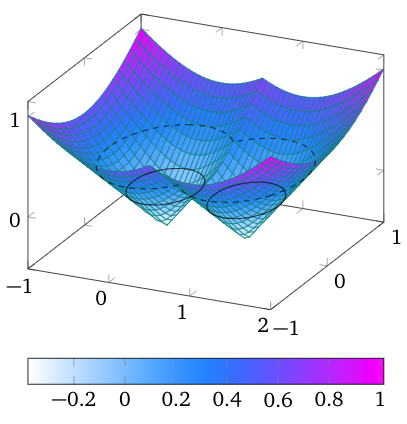
\includegraphics[width=.5\linewidth]{figures/tikz-figures/levelset-function.png}
    \caption[Level set function and iso-contours]{Caption}
    \label{fig:3d-levelset}
\end{figure}

One drawback to the level set method is that instead of solving the equations of motion only for the curve, we increase the complexity when we solve \eqref{eq:general-level-set} for the entire domain. It is still only the curve that is relevant for the solution, and the shape and value of the higher dimensional function are irrelevant. Thus most of the computational resources are then used on calculations that do not affect the curve. 

It is theoretically justified in \cite{MR1100211} and \cite{MR1100206} that the curve is not dependent on the shape of the higher dimensional curve as long as the zero level set is the same. Thus calculations performed on the parts of the domain that do not contain the zero level set are wasteful. For this reason, it has been developed local level set methods that only solve the PDE in a layer around the curve. We refer to \cite{Fast-PDE} for details and implementation of such a local method.





\begin{comment}
What to discuss around the method?
\begin{enumerate}
    \item increased complexity for solving PDE on entire domain. How to fix
    \item Topological flexibility. Situations that are now easily handled.
    \item Existence of viscosity solution (?????). In that case, I must read.
    \item Existence and uniqueness
\end{enumerate}
\end{comment}

\section{Distance Functions}\label{sec:distance-function}

We have now presented the idea behind general level set functions. It was there said that the shape of a higher-dimensional function \uxt\ that implicitly defined the curve, \curve\ was insignificant to the shape and motion of the curve. However, 


it turns out that a \textit{signed distance function} is a natural choice of a higher dimensional function, even though it is not the only choice. This section will present what an unsigned and signed distance function is and why it could be a natural choice for a higher dimensional level set function. 

We begin with the standard distance function, which is everywhere the euclidean distance to an object. We will sometimes call this function \textit{the unsigned distance function} in order to separate it from the signed distance function. 

\begin{definition}[distance function]
\cite{2003-book} A distance function, when applied to a point set, $\pointsetm \in \realspace^d$, yields the minimal euclidean distance from all points $\mathbf{x} \in \realspace^d$ the point set. Thus $d(\mathbf{x}; \pointsetm)$ is defined as 
\begin{equation}
    d(\mathbf{x};\mathcal{V}) = \min_{\mathbf{x}_{v} \in \mathcal{V}} \|\mathbf{x}-\mathbf{x}_{v} \|_2
    \label{eq:unsigned-distance-function}
\end{equation}
When the function $d$ measures the distance to a curve or surface $\Gamma \in \realspace^{d-1}$ it is denoted $d(\mathbf{x}; \Gamma)$ and defined as 
\begin{equation}
    d(\mathbf{x}; \Gamma) = \inf_{\mathbf{x}_{\Gamma}\in \Gamma} \|\mathbf{x}- \mathbf{x}_{\Gamma}\|_2
    \label{eq:unsigned-distance-function-curve}
\end{equation}
\end{definition}

The norm $\|\mathbf{x}-\mathbf{x}_{v} \|$ is positive for all input $\mathbf{x}$ and $\mathbf{x}_{v}$, and thus the distance function is globally positive, or \textit{unsigned}.

The distance function can be computed to an arbitrary point set or curve, and the notion of a distance function makes intuitive sense. Solving the minimization problem can be time consuming, but as long as $\mathcal{V}\neq \emptyset$ or $\Gamma \neq \emptyset$, $d(\mathbf{x},\cdot)$ is uniquely defined everywhere.

Further more, as long as there exists a well defined closest point, the gradient of an unsigned distance function $|\nabla d(\mathbf{x}; \cdot)| = 1$ where $d(\mathbf{x}; \cdot) \in C^1$. The cases where this is not true, is where $\mathbf{x}$ is equidistant from at least two points in the point set , \pointset, or the curve, $\Gamma$, and when $d(\mathbf{x}; \cdot)=0$ \cite{2003-book}.
\begin{comment}
\begin{proposition}[The gradient of a distance function]\label{prop:grad-distance}
For a distance function $d(\mathbf{x};\cdot)$ applied to either a curve or a point set, the following is true.
\begin{equation}
    |\nabla d(\mathbf{x}; \cdot)| = 1, \qquad \forall \mathbf{x} \
    \label{eq:gradient-1}
\end{equation}

\end{proposition}
\begin{proof}
\todo{Skal jeg ta det med her? I appendix? Jeg kan jo ikke referere til deg Anne, men jeg har jo ikke bevist det selv?}
\end{proof}

\end{comment}

We denote the signed distance function $u_d(\mathbf{x}; \cdot)$. In general, the signed distance function both represents the distance to a curve or surface and whether or not a spatial point $\mathbf{x}$ is inside or outside that curve or surface. To construct such a function, we thus need information about where the inside and outside of the curve or surface are. Note that the inside can be established for a closed curve or surface without any prior knowledge, but this is not true for non-closed surfaces or curves. 

The sign of $u_d(\mathbf{x}; \cdot)$ is a discrete value yielding $+1$ if the spatial point is inside the curve or surface and $-1$ if the point is outside. 
\begin{definition}[signed distance function]
In a domain, \domain, including a closed region $\Omega$ with surface or boundary, $\Gamma$, the signed distance function $u_d(\mathbf{x};\Gamma)$ is defined as
\begin{equation*}u_d(\mathbf{x};\Gamma) = \begin{cases} \, d(\mathbf{x}; \Gamma) \qquad & \text{if } \mathbf{x}\in \Omega\\ -d(\mathbf{x}; \Gamma) \qquad & \text{if } \mathbf{x}\in \mathcal{D} \setminus \Omega\end{cases}
\end{equation*}
\label{def:signed-dist}
\end{definition}
These values are exclusively a choice of definition and could as easily be defined oppositely. What is convenient about this definition is that the signed distance function satisfies the conditions \eqref{eq:interior}-\eqref{eq:exterior} concerning the higher dimensional level set function \uxt. A picture showing both the signed and unsigned distance function together can be viewed in \figref{fig:distance-functions}.

\begin{figure}
    \centering
    \includegraphics[width=.5\linewidth]{figures/tikz-figures/signed-distance.tex}
    \caption[Distance Functions]{A cross section of the signed distance function, $u_d(x)$, and the (unsigned) distance function, $d(x)$, applied to a closed curve $\Omega$.}
    \label{fig:distance-functions}
\end{figure}

In addition to being qualified as a level set function, the signed distance function $u_d(\mathbf{x}; \Gamma)$ is a natural choice of level set function for the following reasons. First of all, it can be constructed easily from any initial curve $\Gamma_0$, because signed distance functions are uniquely defined by their zero level set.

In addition they have the property that $|\nabla u_d| = 1$ for all points where $u_d \in C^1$. This comes directly from the same property of unsigned distance functions above and Definition \ref{def:signed-dist}. Also note that the signed distance, $u_d(\mathbf{x}, \Gamma)$ is also $C^1(\Gamma)$ contrary to the unsigned distance $d(\mathbf{x}, \Gamma)$. This can be seen in \figref{fig:distance-functions}.



This property for the gradient is desirable in the level set equation \eqref{eq:general-level-set}, because the absolute value of the gradient decides the sensitivity of the higher dimensional function. This can be seen in \figref{fig:gradient-velocity} by observing that the gradient of the higher dimensional function decides the angle, $\theta$, between the curve and the $x$-axis (or $(x, y)$-plane in $\realspacem^2$) and $v_n \sim \cos (\theta)$.

A steep gradient thus implies a greater angle which again yields smaller $v_n$. Thus a big gradient means that the curve is less sensitive to changes in the higher dimensional function and, conversely, if the gradient is small. This also means that if the gradient is constant everywhere, the sensitivity does not change over the domain, and all level curves will move inwards with speed $v_n$.


\section{Gradient Flow and Derivatives of Domain Integrals} \label{sec:shape-derivatives}
The motivation behind this section is to introduce \textit{gradient flow}, an optimization strategy which will be used to model the general level set equation \eqref{eq:general-level-set} for our situation. We will also see that the gradient flow equation applied to our level set method will rely on transformations produced by velocity fields and their corresponding derivatives. We will thus briefly go through the background and present a useful result concerning derivatives of domain integrals.

We ease into this subject by explaining the concept of gradient flow and how this is related to the level set equation. We remember the level set equation $u_t - v_n|\nabla u|=0$, where the normal speed $v_n$ was the given speed of the zero level set curve. We now want to derive such a speed function to obtain a curve as formulated in the objective of this thesis---a curve with low curvature that approximates a set of sampled points. The velocity field should hence have a normal component that deforms an initial curve gradually until we reach a stationary situation where the objective is fulfilled. In order to construct such a velocity, we must mathematically define our objectives. When we then define the desirable properties as measurable quantities, we can use optimization to find an optimal solution.

We approach this inspired by physics, introducing an energy functional measuring the potential energy of our curve through some properties we want to minimize. Using still the notation from \secref{sec:levelset-methods}, $\Omega(t)$ denotes the area bounded by our curve, \curve. We denote a general energy function for a curve as
\begin{equation}
    E(\Omega(t)) = \int_{\Omega(t)}f(\mathbf{x}) \diff \Omega + \int_{\partial \Omega(t)} g(\mathbf{x})\diff S,
    \label{eq:general-energy}
\end{equation}
where $f$ and $g$ are the measurable quantities of the curve which we want to control.

If we still follow the physical way of thinking, the natural state will minimize the potential energy field and if not affected by other forces, this state will be stationary. A flow in a potential energy field will always move in the direction of fastest falling potential energy and the same idea holds for gradient flow. 

Gradient flow is a continuous version of the well known gradient descent method also known as the steepest descent method. For an optimization problem on the form $\mathbf{x}^* = \argmin_{\mathbf{x}}h(\mathbf{x})$ given an initial guess $\mathbf{x_0}$, where $\mathbf{x}^* \in \realspacem^d$, we improve the solution by following the motion in negative gradient direction, $\mathbf{x}_t = - \nabla h(\mathbf{x})$.

We go back to our energy function $E(\Omega)$. We want to decrease the energy functional by deforming the domain, and that leads to a change in the integration domain $\Omega$. Thus, unlike $h(\mathbf{x})$, the input is not a coordinate in $\realspacem^d$, but a domain of integration $\Omega\subset \realspacem^d$. We thus need to formulate how the energy changes when $\Omega$ is deformed in order to choose the optimal deformation to minimize the energy. We define this change as the derivative of $E$ and denote it $\diff E(\Omega)$.

\begin{figure}
    \centering
    \includegraphics[width=.7\linewidth]{figures/tikz-figures/shape-derivative.tex}
    \caption[Shape transformation by velocity field]{A transformation $T_t$ of a domain $\Omega_0\to\Omega_t$ by flowing in a velocity field $\vv{v}$ over a time $t$. The function $x(t; \mathbf{X})$ describes the path of a material point $\mathbf{X}$ moving in the velocity field.}
    \label{fig:shape-transformation}
\end{figure}

Given a domain $\Omega$ which is assumed to be a bounded, open set in $\realspacem^d$ with a boundary $\Gamma = \partial \Omega\in\realspacem^{d-1}$. A change in the domain into some $\Omega_t$ can be described by a transformation $T_t(\Omega) = \Omega_t$. The velocity method is about describing the domain as a continuum of points where all points are flowing in a velocity field, $\vv{v}$,which perturbs the shape of the domain. Look at \figref{fig:shape-transformation} for reference.

We consider a material point $\mathbf{X}$\todo{Må jeg forklare mat-point?}, moving under the influence of a velocity field $\vv{v}(x, t)$. The trajectory of the material point, $\mathbf{X}$, in Eulerian coordinates is denoted $x(t; \mathbf{X})$, and will follow the velocity field $\vv{v}(x, t)$. From this, we get the differential equation for the movement of the material points
\begin{equation*}
    \frac{\diff x}{\diff t} (\mathbf{X}, t) = \vv{v}(x(t; \mathbf{X}), t), \quad x(t; \mathbf{X})=\mathbf{X}, \quad t \geq 0.
\end{equation*}

The transformation, $T_t$, thus moves the material points along their trajectories given by the velocity field, which mathematically can be formulated as
\begin{equation}
    \mathbf{X} \mapsto T_t(\mathbf{X}; \vv{v}) = x(t; \mathbf{X}).
    \label{eq:euler-lagrange}
\end{equation}

For the domain $\Omega$, the transformation moves all material points in $\Omega$ along their respective trajectories. The time $t$ in the transformation, $T_t$, represents how long we move along the trajectories. This means that $T_0(\Omega) = \Omega$, or in other words, $T_0 = I$. When $t\neq 0$, the total shape transformation of $\Omega_0$ along a velocity field, $\vv{v}$, is denoted as follows
\begin{equation}
    \Omega_t(\vv{v}) = T_t(\vv{v})(\Omega_0) = \{T_t(\mathbf{X}; \vv{v}), \quad \forall \, \mathbf{X} \in \Omega_0 \} .
    \label{eq:tot-shape-trans}
\end{equation}

We have now introduced the notation we need to introduce derivatives of domain integrals. The following proposition and the proof can be found in a more general version in the book "Introduction to Shape Optimization" by J. Sokolowski and J. Zolesio \cite{zolesio-MR1215733}. 

\begin{proposition}
Let $\Omega(t)$ be a smooth domain in $\realspacem^2$ bounded by the boundary curve $\Gamma$. Define the functions $f(\mathbf{x})\in W^{1, 1}(\realspacem^2)$ and $g(\mathbf{x})\in W^{2, 1}(\realspacem^2)$ not dependent on the domain of integration, $\Omega(t)$. Define the functions $J_1$ and $J_2$:
\begin{align*}
    J_1(\Omega(t)) &= \int_{\Omega(t)} f(\mathbf{X}) \diff \Omega \\
    J_2(\Omega(t)) &= \int_{\Gamma(t)} g(\mathbf{X}) \diff S(\Gamma).
\end{align*}
Let the the velocity field $\vv{v}$ be continuous. The derivatives of $J_1$ and $J_2$ with respect to the integration domain at a fixed time $t=t^*$ is then

\begin{align}
    \diff J_1(\Omega(t^*)) &= \int_{\Gamma(t^*)}f(\mathbf{X}) (\vv{v}(t^*)\cdot \vv{n}) \diff \Gamma, \label{eq:J1-der}\\
    \diff J_2(\Omega(t^*)) &= \int_{\Gamma(t^*)} \big(\frac{\partial}{\partial \vv{n}}g(\mathbf{X}) + \kappa g(\mathbf{X}) ) (\vv{v}(t^*)\cdot \vv{n} \big) \diff S(\Gamma). \label{eq:J2-der}
\end{align}
\label{prop:shape-derivative}
\end{proposition}

Now, returning to gradient flow, we need to find the direction of $\vv{v}(t)$ from Proposition \ref{prop:shape-derivative} that maximizes $dE(\Omega)$ and move in the opposite direction. Since the gradient is dependent on the inner product $\vv{v}(t)\cdot \vv{n}$, the direction of maximal derivative is when $\vv{v}(t)$ parallel to $\vv{n}$. For our general energy function $E(\Omega)$ this means that the curve velocity $\Gamma_t$ following gradient flow will have speed
\begin{equation}
    \Gamma_t = -v_n \vv{n}_{\Gamma} = -(f(\mathbf{x}) + g(\mathbf{x})) \vv{n}_{\Gamma}.
    \label{eq:optimal-descent}
\end{equation}


%%%%%%%%%%%%%%%%%%%%%%%%%%%%%%%%%%%%%%%%%%%%%%%%%%%%%%%%%%%%%%%%%%%%%%%%%%%%%%%%%%

\begin{comment}
\begin{proposition}
Let $\Omega$ be a smooth domain in $\realspacem^2$ bounded by the boundary curve $\Gamma$. Define the functions $f(\Omega)\in W^{1, 1}(\realspacem^2)$ and $g\in W^{1, 1}(\realspacem^2)$. Define the functions $J_1$ and $J_2$:
\begin{align*}
    J_1(\Omega) &= \int_{\Omega} f(\Omega) \diff x \\
    J_2(\Omega) &= \int_{\Gamma} g(\Omega) \diff S(\Gamma).
\end{align*}
Let the the velocity field $\vv{V}$ be continuous. The derivatives of $J_1$ and $J_2$ with respect to the integration domain is then

\begin{align}
    J_1'(\Omega) &= \int_{\Omega}f'(\Omega; \vv{V})\diff x + \int_{\Gamma}f(\Omega) (\vv{V}(0)\cdot \vv{n}) \diff \Gamma \label{eq:J1-der}\\
    J_2'(\Omega) &= \int_{\Gamma} g'(\Omega; \vv{V})|_{\Gamma}\diff S(\Gamma) + \int_{\Gamma} \big(\frac{\partial}{\partial \vv{n}}g(\Omega) + \kappa g(\Omega) ) (\vv{V}(0)\cdot \vv{n} \big) \diff S(\Gamma) \label{eq:J2-der}
\end{align}
where $f'(\Omega; \vv{V})$ and $g'(\Omega; \vv{V})$ are the shape derivatives of $f$ and $g$ \cite{zolesio-MR1215733}.
\label{prop:shape-derivative}
\end{proposition}
\begin{proof}
The proof relies on the theory of shape derivatives and for a full proof we refer to \cite{zolesio-MR1215733}. We can nevertheless present the idea given the defined notation.

Using the definition of the derivative, we can write $J_1'(\Omega)$ as
\begin{align*}
    J_1'(\Omega) &= \lim_{t\downarrow 0} \frac{J_1(\Omega_t)-J_1(\Omega)}{t} \\
    &=\lim_{t\downarrow 0} \frac{\int_{\Omega_t} f(\Omega_t) \diff x-\int_{\Omega} f(\Omega) \diff x}{t}.
\end{align*}


We use \eqref{eq:euler-lagrange} to do a change of variable to express the integral over $\Omega_t$ in terms of $\Omega$. We write $x=T_t(\vv{V})(\mathbf{X})$ and use the substitution rule to obtain
\begin{equation*}
    J_1(\Omega_t) = \int_{\Omega} \text{det}(D T_t)f(T_t(\Omega)) \diff x,
\end{equation*}
where $DT_t$ is the Jacobian matrix of the transformation $T_t(\vv{V})$. We also express $\Omega$ as $\Omega_t|_{t=0}$ and for $T_t|_{t=0}$, the transformation is only the identity mapping. It can also be shown that $\text{det}(D T_0) = \nabla \cdot \vv{V}(0)$ \cite{zolesio-MR1215733}.
\begin{equation*}
    J_1'(\Omega) = \lim_{t\downarrow 0} \frac{\int_{\Omega} \text{det}(D T_t)f(T_t(\Omega)) \diff x-\int_{\Omega} \nabla \cdot \vv{V}(0)f(\Omega_t)\diff x}{t}.
\end{equation*}
Given a continuous transformation $T_t$ with a differentiable Jacobian, $\text{det}(DT_t)$, it can be shown that this is equal to \cite{zolesio-MR1215733}

\begin{equation*}
    J_1'(\Omega; \vv{V}) = \int_{\Omega} f'(\Omega; \vv{V}) \diff x +\int_{\Omega} \nabla \cdot (f(\Omega)\vv{V}(0) ) \diff x.
\end{equation*}
Using the divergence theorem on the last term, yields \eqref{eq:J1-der}.

The proof of \eqref{eq:J2-der} is performed in a similar manner, doing a change of variables and using a substitution rule. However, it demands some new definitions and concepts, so we do not recite it here.


For the integral function $J_2$, we similarly write
\begin{align*}
    J_2'(\Omega) &= \lim_{t\downarrow 0} \frac{J_2(\Omega_t)-J_2(\Omega)}{t} \\
    &= \lim_{t\downarrow 0} \frac{\int_{\Gamma_t}g(\Gamma_t) \diff \Gamma-\int_{\Gamma} g(\Gamma) \diff \Gamma}{t}.
\end{align*}
Again we perform the change of variable $x=T_t(\vv{V})(\mathbf{X})$. For a proof of the next equation, we refer to Proposition 2.47 in \cite{zolesio-MR1215733}.

\begin{equation*}
    J_2(\Omega) = \int_{\Gamma}g(\Gamma_t)\circ T_t \omega(t) \diff \Gama.
\end{equation*}


Now we have the tools we need in order to minimize the energy function $E(\Omega)$ using gradient flow. Then we can move on to the modeling aspect of this thesis.
    
\end{proof}

\end{comment}


\clearpage
%\subsection{The Eikonal equation}
The Eikonal equation is closely tied with distance functions, or more accurately, it turns out that distance functions are solutions of the Eikonal equation. 

For an expanding front, $\Gamma$, moving outwards with speed $F>0$, we can compute the arrival time at a point $(x, y)$, denoted $T(x, y)$. The initial front is then $T(x, y)=0$, and it grows with rate $F$ outwards, since the distance traveled $d$ given a velocity $F$ and time $T$ is $d=FT$ and thus $\diff d/\diff t=F$ and $1=F \nabla T$ and we get
\begin{equation}
    \begin{aligned}
        &|\nabla T| = \frac{1}{F} \\
        &T(x, y)=0 \qquad \text{for } (x, y) \in \Gamma, 
    \end{aligned}
    \label{eq:eikonal-equation}
\end{equation}
which is the Eikonal equation \cite{sethian1999level}. We observe that for $F=1$, this is $|\nabla T|=1$ and from Proposition \ref{prop:grad-distance}, we see that the gradient of the distance function must satisfy the Eikonal equation \eqref{eq:eikonal-equation}. This is intuitive because the relation between the distance and time is $s=FT$ and this a velocity $F=1$ would mean that the distance traveled must be equal to the travel time used with speed 1.

It is this relation to the distance function that makes the Eikonal equation interesting in this setting. In stead of looking at the construction of a distance problem as a minimization problem, we solve the Eikonal equation. 

\begin{comment}
\begin{enumerate}
    \item Relation to Hamilton Jacobi and Level set formulation
    \item Distance function - stupid approach :-) vs idea behind fast marching - boundary moving with speed 1.
    \item Algorithm for FMM??
\end{enumerate}
\end{comment}


\clearpage


